\documentclass[12pt]{article}
\usepackage{latexblog}

% ============================================================
% Blog Metadata
% ============================================================
\blogtitle{Vert.X(1)：简介}
\blogdate{2020-12-07}
\blogtags{Vert.X, 框架, 闲话编程}
\bloglang{zh}
\blogsummary{}

\begin{document}
\makeblogtitle

最开始了解到Vert.X是在\href{https://www.techempower.com}{Web Framework Benchmarks}中看到，性能超群的一个web框架，但说实话知名度不是特别高。

\begin{figure}
\centering
\pandocbounded{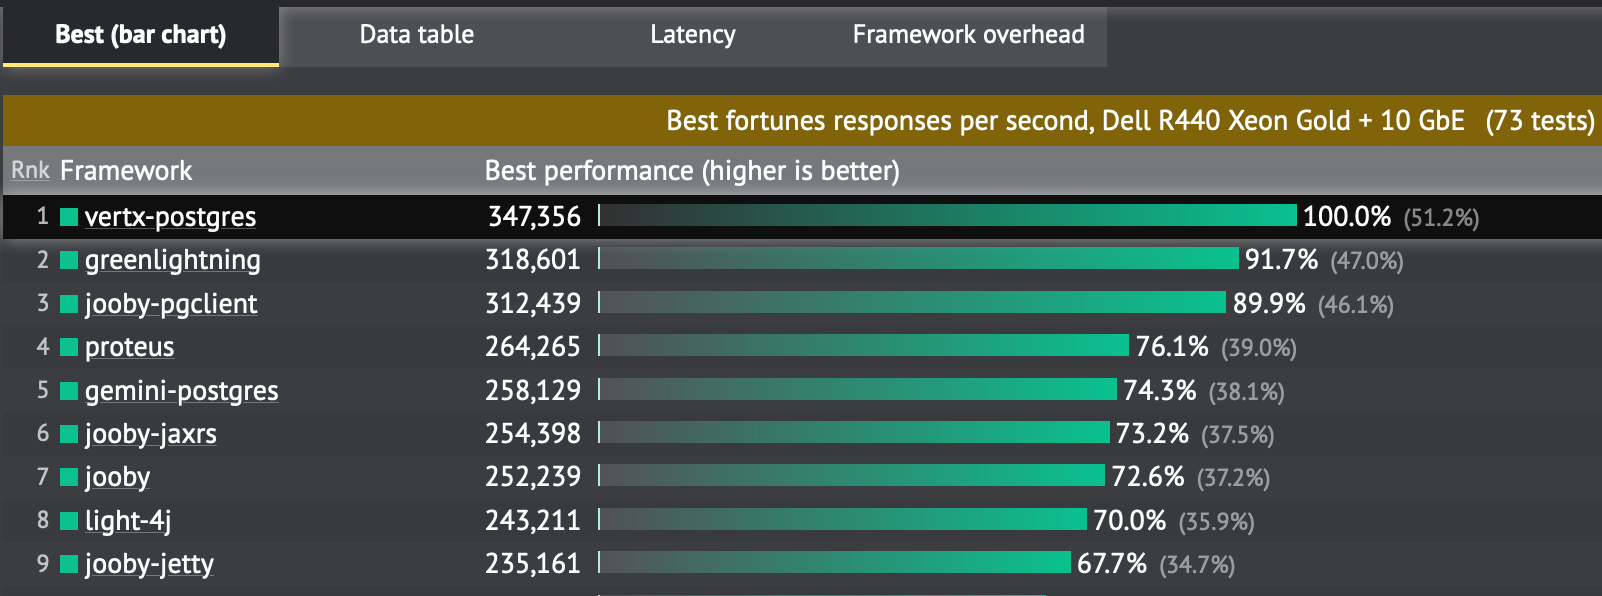
\includegraphics[keepaspectratio,alt={Vert.X Benchmark}]{images/Vert.x_Benchmark.png}}
\caption{Vert.X Benchmark}
\end{figure}

而官网介绍也谦逊的很，甚至都说自己不算一个web框架，而是一个''tool-kit''：

\begin{quote}
Eclipse Vert.x is a tool-kit for building reactive applications on the JVM.
\end{quote}

\section{特点}\label{ux7279ux70b9}

Vert.x采取的是事件驱动的非阻塞异步响应模型，而不是类似Servlet一样为每一个连接分配一个新的线程。这样做的好处就是可以利用少量的线程处理很多的并发连接。而采取blocking IO的线程在等待IO操作完成的时候，线程会被挂起，而后唤醒。但是这个操作本身也是有一定的开销的，当线程数很大的时候这个开销就尤为明显。

简单来说，Vert.x就是JVM版本的NodeJS，但一个比较大的区别就是NodeJS是单线程模型的，而Vert.x可以有多个event loop，因此能够更加有效的利用多核的优势。

Vert.x的另一个特点就是提供了多种语言的绑定（并不仅仅是简单的wrap一下，而且充分利用了各个语言的特点）：

\begin{itemize}
\tightlist
\item
  Java
\item
  JavaScript
\item
  Groovy
\item
  Ruby
\item
  Kotlin
\item
  Scala
\end{itemize}

\subsection{什么是响应式（Reactive）}\label{ux4ec0ux4e48ux662fux54cdux5e94ux5f0freactive}

根据\href{https://www.reactivemanifesto.org/}{The Reactive Manifesto}的定义，一个响应式的系统具有四个特点： \pandocbounded{\includesvg[keepaspectratio]{https://www.reactivemanifesto.org/images/reactive-traits.svg}}

\begin{itemize}
\tightlist
\item
  Responsive：The system responds in a timely manner if at all possible.
\item
  Resilient：The system stays responsive in the face of failure.
\item
  Elastic: The system stays responsive under varying workload.
\item
  Message-driven: Reactive Systems rely on asynchronous message-passing to establish a boundary between components that ensures loose coupling, isolation and location transparency.
\end{itemize}

\subsection{组件}\label{ux7ec4ux4ef6}

Vert.x又包含了很多个部分：

\subsubsection{Web组件}\label{webux7ec4ux4ef6}

\begin{itemize}
\tightlist
\item
  Core: 包含底层的Http/TCP、文件等的访问功能。
\item
  Web: 可以用来创建Web应用和微服务
\item
  Web Client: http请求客户端
\item
  Web API Contract: 用来实现契约先行的开发模式以及契约测试
\item
  其他: Web API Service, Web GraphQL Handler等，不过目前都还在Technical Preview阶段
\end{itemize}

\subsubsection{数据访问}\label{ux6570ux636eux8bbfux95ee}

数据访问组件提供了一系列的异步访问client，当然也可以直接使用原始的数据库驱动。支持的数据库有：

\begin{itemize}
\tightlist
\item
  MongoDB client
\item
  Redis client
\item
  Cassandra client
\item
  SQL Common
\item
  JDBC client
\item
  Reactive MySQL/DB2/PostgreSQL client(Technical preview)
\end{itemize}

\subsubsection{Reactive}\label{reactive}

提供了各种创建响应式应用程序的组件。

\begin{itemize}
\tightlist
\item
  Vert.x Rx: 不喜欢回调可以使用RxJava风格的API
\item
  Reactive streams: 可以与Akka/Project Reactor等其他reactive系统交互
\item
  Vert.x Sync: 用来部署使用fiber(纤程，一种轻量级的线程)的节点，可以编写串行化风格的代码
\item
  Kotlin coroutines: 携程的支持，可以使用\texttt{async/await}或者channels。
\end{itemize}

\subsubsection{Microservices}\label{microservices}

创建微服务的组件：

\begin{itemize}
\tightlist
\item
  service discovery
\item
  circuit breaker
\item
  config
\end{itemize}

\subsubsection{MQTT}\label{mqtt}

提供了MQTT的server和client端组件。

\subsubsection{Authentication and Authorisation}\label{authentication-and-authorisation}

认证授权相关：

\begin{itemize}
\tightlist
\item
  Auth common
\item
  JDBC auth
\item
  JWT auth
\item
  Shiro auth
\item
  MongoDB auth
\item
  OAuth2
\item
  .htdigest Auth
\end{itemize}

\subsubsection{Messaging}\label{messaging}

\begin{itemize}
\tightlist
\item
  AMQP client(Technical preview)
\item
  STOMP client \& Server
\item
  RabbitMQ client
\item
  AMQP bridge
\end{itemize}

\subsubsection{其他}\label{ux5176ux4ed6}

\begin{itemize}
\tightlist
\item
  Kafka client
\item
  Mail client: SMTP 客户端
\item
  Consul client
\item
  JCA Adaptor
\item
  Event Bus bridge:TCP/Apache camel
\item
  Health check
\item
  Metrics
\item
  Shell
\item
  Docker
\item
  Vert.x Unit
\item
  \ldots{}
\end{itemize}

\section{使用}\label{ux4f7fux7528}

\subsection{Hello World}\label{hello-world}

\begin{Shaded}
\begin{Highlighting}[]
\KeywordTok{public} \KeywordTok{class}\NormalTok{ VertxEcho }\OperatorTok{\{}
    \KeywordTok{public} \DataTypeTok{static} \DataTypeTok{void} \FunctionTok{main}\OperatorTok{(}\BuiltInTok{String}\OperatorTok{[]}\NormalTok{ args}\OperatorTok{)} \OperatorTok{\{}
\NormalTok{        Vertx vertx }\OperatorTok{=}\NormalTok{ Vertx}\OperatorTok{.}\FunctionTok{vertx}\OperatorTok{();}

\NormalTok{        vertx}\OperatorTok{.}\FunctionTok{createNetServer}\OperatorTok{()}
            \OperatorTok{.}\FunctionTok{connectHandler}\OperatorTok{(}\NormalTok{socket }\OperatorTok{{-}\textgreater{}} \OperatorTok{\{}
\NormalTok{                socket}\OperatorTok{.}\FunctionTok{handler}\OperatorTok{(}\NormalTok{buffer }\OperatorTok{{-}\textgreater{}} \OperatorTok{\{}
\NormalTok{                    socket}\OperatorTok{.}\FunctionTok{write}\OperatorTok{(}\StringTok{"Hello:"} \OperatorTok{+}\NormalTok{ buffer}\OperatorTok{);}
                \OperatorTok{\});}
            \OperatorTok{\})}
            \OperatorTok{.}\FunctionTok{listen}\OperatorTok{(}\DecValTok{3000}\OperatorTok{);}
    \OperatorTok{\}}
\OperatorTok{\}}
\end{Highlighting}
\end{Shaded}


\end{document}
